% Type of the document
\documentclass{beamer}

% elementary packages:
\usepackage{graphicx}
\usepackage[latin1]{inputenc}
\usepackage[T1]{fontenc}
\usepackage[english]{babel}
\usepackage{listings}
\usepackage{xcolor}
\usepackage{eso-pic}
\usepackage{mathrsfs}
\usepackage{url}
\usepackage{amssymb}
\usepackage{amsmath}
\usepackage{multirow}
\usepackage{hyperref}
\usepackage{booktabs}

% additional packages
\usepackage{bbm}

% packages supplied with ise-beamer:
\usepackage{cooltooltips}
\usepackage{colordef}
\usepackage{beamerdefs}
\usepackage{lvblisting}
% logobig and logosmall are the internal names for the pictures: do not modify them. 
% Pictures must be supplied as JPEG, PNG or, to be preferred, PDF
\pgfdeclareimage[height=4.5cm]{logobig}{LogoIRTG}
% Supply the correct logo for your class and change the file name to "logo". The logo will appear in the lower
% right corner:
\pgfdeclareimage[height=0.7cm]{logosmall}{MSM_AN.png}

% Title page outline:
% use this number to modify the scaling of the headline on title page
\renewcommand{\titlescale}{1.0}
% the title page has two columns, the following two values determine the percentage each one should get
\renewcommand{\titlescale}{1.0}
\renewcommand{\leftcol}{0.6}

% Define the title.Don't forget to insert an abbreviation instead 
% of "title for footer". It will appear in the lower left corner:
\title[Solutions to Quizzes]{Solutions to Quizzes}
% Define the authors:
\authora{Ya Qian} % a-c
\begin{document}
% Define any internet addresses, if you want to display them on the title page:
\def\linka{lvb.wiwi.hu-berlin.de}
\def\linkb{\\case.hu-berlin.de}
\def\linkc{\\irtg1792.hu-berlin.de}
% Define the institute:
\institute{Ladislaus von Bortkiewicz Chair of Statistics\\
C.A.S.E. -- Center for Applied Statistics\\
and Economics\\
Humboldt--Universit\"at zu Berlin\\}

% Comment the following command, if you don't want, that the pdf file starts in full screen mode:
\hypersetup{pdfpagemode=FullScreen}

%Start of the document
\begin{document}

% create the title slide, layout controlled in beamerdefs.sty and the foregoing specifications
\frame[plain]{
\titlepage
}
%%%%%%%%%%%%%%%%%%%%%%%%%%%%%%%%%%%%%%%%%%%%%%%%%%%%%%%%%%%%%%%%%%%%%%%%%%%%%%%%%%%%%%%%%%%%%%%%%%%%%%%%%%%%%%%%%%%%%%%%
\section{Solution to Quizzes}
%%%%%%%%%%%%%%%%%%%%%%%%%%%%%%%%%%%%%%%%%%%%%%%%%%%%%%%%%%%%%%%%%%%%%%%%%%%%%%%%%%%%%%%%%%%%%%%%%%%%%%%%%%%%%%%%%%%%%%%%
\frame{
\frametitle{Quiz 11: If $X_n$ is $\operatorname{AN}(\mu_n, \sigma_{n}^2)$, then so is $\frac{n-1}{n}X_n$, but NOT $\frac{n^{1/2}-1}{n^{1/2}}X_n$, why? and find a $r.v. X_n s.t. X_n \sim \operatorname{AN}(n, 2n)$}
Proof: \\
According to Lemma 23, if $X_n$ is $\operatorname{AN}(n, 2n)$, then also $a_nX_n+b_n$ is 
$\operatorname{AN}(n, 2n) \iff a_n \rightarrow 1, \frac{\mu_n(a_n-1)+b_n}{\sigma_n} \rightarrow 0$.
\begin{itemize}
\item For $\frac{n-1}{n}X_n$:\\
$a_n=\frac{n-1}{n}, b_n=0,$ we have obviously \\
$a_n=\frac{n-1}{n} \rightarrow 1, \frac{\mu_n(a_n-1)+b_n}{\sigma_n}=\frac{n(\frac{n-1}{n}-1)+0}{\sqrt{2n}}=\frac{-1}{\sqrt{2n}}\rightarrow 0$\\
By Lemma 23, $\frac{n-1}{n}X_n$ is also $\operatorname{AN}(n, 2n)$.
\end{itemize} }
}

\frame{
\frametitle{Quiz 11: If $X_n$ is $\operatorname{AN}(\mu_n, \sigma_{n}^2)$, then so is $\frac{n-1}{n}X_n$, but NOT $\frac{n^{1/2}-1}{n^{1/2}}X_n$, why? and find a $r.v. X_n s.t. X_n \sim \operatorname{AN}(n, 2n)$}
Proof:\\
\begin{itemize}
\item For $\frac{n^{1/2}-1}{n^{1/2}}X_n$:\\
$a_n=\frac{n^{1/2}-1}{n^{1/2}}, b_n=0,$ we have obviously\\
$a_n=\frac{n^{1/2}-1}{n^{1/2}} \rightarrow 1, \frac{\mu_n(a_n-1)+b_n}{\sigma_n}=\frac{n(\frac{n^{1/2}-1}{n^{1/2}}-1)+0}{\sqrt{2n}}=-\sqrt{2}/2 \nrightarrow 0$\\
By Lemma 23, $\frac{n^{1/2}-1}{n^{1/2}}$ is not $\operatorname{AN}(n, 2n)$.
\end{itemize} 
}

\frame{
\frametitle{Quiz 11: If $X_n$ is $\operatorname{AN}(\mu_n, \sigma_{n}^2)$, then so is $\frac{n-1}{n}X_n$, but NOT $\frac{n^{1/2}-1}{n^{1/2}}X_n$, why? and find a $r.v. X_n s.t. X_n \sim \operatorname{AN}(n, 2n)$}
An example $r.v. X_n$ satisfies $X_n \sim \operatorname{AN}(n, 2n)$
\begin{center}
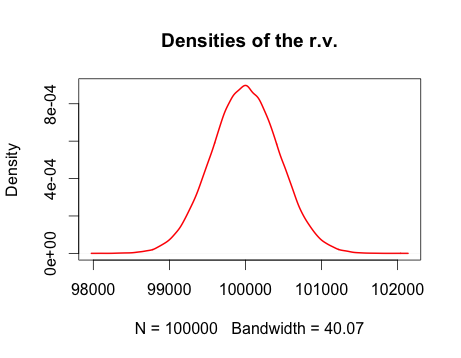
\includegraphics[scale=0.25]{MSM_AN.png}
\end{center}
	\begin{center}	\href{https://github.com/xuxiu/MSMquiz/tree/master/Quiz11_p5-15}{\quantnet Quiz11-MSM.R}
    \end{center}
}

\end{document}